%%%%%%%%%%%%%%%%%%%%%%%%%%%%%% -*- Mode: Latex -*- %%%%%%%%%%%%%%%%%%%%%%%%%%%%
%% project.modeling.tex --
%% Author          : Philip Johnson
%% Created On      : Fri Jan 13 07:58:21 2012
%% Last Modified By: Alek Kavcic
%% Last Modified On: Mon Jan 25 16:35:19 2012
%%%%%%%%%%%%%%%%%%%%%%%%%%%%%%%%%%%%%%%%%%%%%%%%%%%%%%%%%%%%%%%%%%%%%%%%%%%%%%%

\subsubsection{Modeling and analysis}

Given appropriate data, the next step is to apply analytic techniques to
create real-time and historical information useful for control and
optimization of the microgrid.

Two important contributions of this part of the research will be: (1)
analytic techniques that enable us to adequately characterize the current
state of the microgrid without a cost-prohibitive deployment of sensing
equipment, and (2) analytic techniques that enable short-term prediction of
various useful attributes of the micro-grid (such as future (potentially
peak) load and ramp) and the surrounding environment (insolation, wind
speed and direction, etc.)

It should be noted that there is an interdependence between the ``sensing
and monitoring'' subproject and the ``modeling and analysis'' subproject:
we will ``tune'' the installation of sensing equipment in order to obtain
acceptable quality of analytic outcomes for the next step, control and
optimization. Furthermore, the chosen models and analytical tools cannot
only be good descriptors of the underlying physical processes, but also
need to be matched to the signal processing (detection and estimation)
methods, or else the signal processing methods will not be of much use.


\begin{figure}[t]
  \begin{center}
   \includegraphics[width=0.9\textwidth]{Bipartite.eps}
   \caption{\label{B} Factor graph - an abstraction of the microgrid.
       The factor graph consists
       of the behavior layer and the observation layer. The
       communication layer provides additional global
       communication features. In this figure, the state
       variables are denoted by $x_i$ and available observations
       (sparse measurements) are denoted by $y_i$.
       The belief-propagation algorithm is
       a monitoring algorithm that works by passing only {\em local}
       messages along the solid edges of the graph, yet achieves {\em global}
       monitoring.}
  \end{center}
\end{figure}

\paragraph{Belief Propagation.} Through or previously funded NSF project
(ECCS-1029081), we have already established that the factor-graph approach
is well-suited to modeling the electrical connections of a microgrid.
Figure~\ref{B} shows a schematic view of a factor-graph associated with a
fictitious microgrid. The nodes in the mocrogrid are divided into three
layers: 1) the observation layer (sensors, measurement equipment), 2) the
behavior layer (collection of network nodes, loads and microgenerators) and
3) the communication layer. We demonstrated that, with only a few well
placed sensors in the grid, we are able to track slowly evolving behaviors
of the grid as well as with more elaborate exact maximum-likelihood
estimators~\cite{Hu10,Hu11,Hu11a}. This is mainly because the electrical
grid is typically a {\em tree} graph, where correlations among renewable
sources create rare loops with large diameters.

In this research, we plan to use belief propagation as a tool that would
also enable 1) tracking the grid in transitional modes (e.g., if a large
number of users and/or renewable microgenerators enter and/or drop from the
microgrid abruptly) and 2) short-term future prediction of the grid
behavior at node-levels.  To this end, we will develop the necessary
modeling and prediction tools.

\paragraph{Modeling demand.} Often, the demand in grid networks is
described using historical {\em histograms}. However, historical histogram
patterns do not reveal the true spatiotemporal character of the demand. It
is obvious that spatial and temporal correlations will need to be exploited
in order to arrive at a model that would be useful for spatiotemporal
demand prediction, i.e., prediction that can predict the demand, say, 5
minutes in advance at any given set of spatial location locations in the
microgrid.  Furthermore, in order to utilize the belief-propagation tool,
we will seek to model the demand among various nodes in the microgrid as a
spatiotemporal Markov process with as few loops as possible (because it is
the loops that adversely affect belief
propagation~\cite{Wiberg95,Kschischang01,Loeliger07}). We note that simple
Gauss-Markov process modeling will likely not suffice because Gaussian
processes are well-suited only for tracking slow changes.  Yet, demand in
campus environment can be spatially and temporally bursty (because of
correlation to class-times tarts, lab-clusters, weather/heat conditions and
distributed renewable microgenerators).  For this reason, we plan leverage
our experience in modeling Gauss-Markov processes~\cite{Kavcic00a} and
finite-state machines~\cite{Yang05,Vontobel08} to develop a comprehensive
double-layer Gauss-Markov/finite-state spatiotemporal demand model.  We
will extrapolate, calibrate and test the model using measurement data from
sensors distributed around the campus.

\paragraph{Modeling renewable sources.} Much like the loads (demand) are
spatially and temporally distributed, so are the renewable
micro-generators. The UH campus already has several clusters of
photovoltaic (PV) generators and two small wind turbines (typically used
for experimental purposes) dispersed around campus. Therefore, we will need
to model their energy outputs using spatiotemporal Markov processes (with
as few loops as possible) that are capable of modeling both slowly varying
effects as well as (spatially and temporally) localized bursts. Again, we
will utilize a layered Gauss-Markov/finite-state modeling approach to
capture both effects.  However, unlike modeling demand, here we will need
to heavily correlate the model to weather conditions (night/day,
cloud-cover, wind speed and direction). We will extrapolate, calibrate and
test the model using weather measurement data from irradiance sensors, wind
velocity sensors and cloud cameras distributed around the campus.


\paragraph{Prediction.} It is a well-known fact that the Kalman predictor
is the optimal predictor of spatial and temporal Gaussian
processes~\cite{Kalman60,Kalman_Bucy61,Kailath68}. When the Gaussian
process further possesses a Markov structure (i.e., a Gauss-Markov
process), the Kalman predictor is computationally less
intensive~\cite{Kschischang01,Loeliger07}. In our case, we will
likely have a two-layer spatial and temporal
Gauss-Markov/finite-state process to track. The optimal tracker of
this process would be a spatiotemporal combination of a Kalman
predictor~\cite{Kalman60,Kalman_Bucy61} and a forward recursion of
the Baum-Welch algorithm~\cite{Baum66,Bahl74}. However, this
approach will likely be too computationally intensive to be
practical. Therefore, we will ignore the loops in the model, and
implement the predictor using belief propagation derived for a
tree-like double-layer (Gauss-Markov/finite-state) graph, but
applied to the exact loopy microgrid graph.

We envision that the developed prediction tool will be used to
indicate where and how the control mechanisms (e.g., peak-shaving,
gray-outs, etc.) should be applied. However, we must consider the
sensitivity of certain locations when applying control.  For
example, it would be detrimental to shut off the air conditioner in
a sensitive climate controlled laboratory, or in computer server
clusters that must remain cool. For this reason, it is desirable to
have a prediction method that will account for these sensitivities.
It is well-known that any prediction method suffers form
uncertainly, misdetection and false alarms. Grossly false estimation
or prediction of the state of certain sensitive nodes may adversely
affect the stability of the network or sensitive campus locations.
This can be minimized in two possible ways. Firstly, we may choose
to place sensors in the vicinities of highly sensitive nodes, and
thus minimize the risk of misprediction. Secondly, we may choose to
dampen the belief-propagation algorithm to prevent wild belief
swings in the vicinities of highly sensitive nodes. This amounts to
placing weights (or other types of constraints) on beliefs
corresponding to highly sensitive nodes. We shall term this approach
{\em sensitivity weighted} belief-propagation. To our knowledge, no
such approach has been attempted in smart-grid networks, although
similar strategies are available in the communications and
error-control coding literature~\cite{Wang99,Jiang06a,Varnica07}.

\paragraph{Analysis.} The final piece of the modeling and analysis effort
is the actual analysis of the proposed models and tracking methods. In
tracking mode, we will utilize statistical signal processing techniques to
analyze the performance of the trackers.  For example, under under
stationarity conditions, we can easily bound the performance of
maximum-likelihood estimators of Gausian processes. We will extend these
techniques, and combine them with bounding techniques typical for
finite-state processes~\cite{Huang09}, to develop bounds for tracking the
layered Gauss-Markov/finite-state process in under certain stationarity assumptions.

Under extremely non-stationary conditions, however, it will be
extremely difficult to come up with analytical tools that will be
able to bound the performance of the estimator/tracker. Indeed, in
the signal processing literature, response to extreme
non-stationarities are typically demonstrated by
simulations~\cite{Yang95,Tanaka05}. For this reason, it is actually
very important to design a good model that will not only be useful
for designing the detector, but also for designing the simulator.
The usefulness of this approach will be extremely important when
determining the response to {\em rare events}. Rare events are
events that are rarely (or never observed) in practice until they
happen in reality (e.g., black-outs, shut-downs, catastrophic
failures). The only way to understand how such events would affect
the system is through simulations. We will conduct analysis studies
of these rare, extremely non-stationary events through the means of
simulations using the developed process models.
